% docs/slides/preamble.tex -- 五份 deck 共享
\documentclass[aspectratio=169,11pt]{beamer}

% ==== 中文与字体 ====
\usepackage[UTF8,fontset=none]{ctex}
\usepackage{fontspec}

\IfFontExistsTF{PingFang SC}{%
  \setCJKmainfont{PingFang SC}[BoldFont=PingFang SC,ItalicFont=PingFang SC,AutoFakeSlant=0.15]
  \setCJKsansfont{PingFang SC}[ItalicFont=PingFang SC,AutoFakeSlant=0.15]
  \setCJKmonofont{PingFang SC}
}{%
  \IfFontExistsTF{Source Han Sans SC}{%
    \setCJKmainfont{Source Han Sans SC}
    \setCJKsansfont{Source Han Sans SC}
  }{%
    \IfFontExistsTF{Noto Sans CJK SC}{%
      \setCJKmainfont{Noto Sans CJK SC}
      \setCJKsansfont{Noto Sans CJK SC}
    }{%
      \setCJKmainfont{Heiti SC}
      \setCJKsansfont{Heiti SC}
    }
  }
}

\IfFontExistsTF{Helvetica Neue}{\setmainfont{Helvetica Neue}}{%
  \IfFontExistsTF{Inter}{\setmainfont{Inter}}{}}
\IfFontExistsTF{JetBrains Mono}{\setmonofont{JetBrains Mono}[Scale=0.85]}%
  {\setmonofont{Menlo}[Scale=0.85]}

% ==== 颜色 ====
\usepackage{xcolor}
\definecolor{cMain}{HTML}{1F4E79}
\definecolor{cAccent}{HTML}{E07A1F}
\definecolor{cGray}{HTML}{595959}
\definecolor{cMute}{HTML}{F4F4F4}
\definecolor{cOK}{HTML}{2E7D32}
\definecolor{cBad}{HTML}{B23A3A}
\definecolor{cWarn}{HTML}{C8A300}

% ==== 主题 ====
\usepackage{tcolorbox}
\usetheme{metropolis}
\metroset{progressbar=frametitle,numbering=fraction,block=fill}
\setbeamercolor{frametitle}{bg=cMain,fg=white}
\setbeamercolor{progress bar}{fg=cAccent,bg=cMute}
\setbeamercolor{alerted text}{fg=cAccent}
\setbeamercolor{title}{fg=cMain}

% metropolis 默认尝试 Fira Sans，未安装时 fallback 到 Latin Modern Sans。
% 这里在主题加载后显式覆盖，强制使用 macOS 上一定存在的 Helvetica Neue，
% 跟中文 PingFang 风格一致；找不到则按顺序尝试 Inter / Arial。
\IfFontExistsTF{Helvetica Neue}{%
  \setsansfont{Helvetica Neue}%
}{%
  \IfFontExistsTF{Inter}{\setsansfont{Inter}}{%
    \IfFontExistsTF{Arial}{\setsansfont{Arial}}{}}%
}

% ==== TikZ ====
\usepackage{tikz}
\usetikzlibrary{positioning,arrows.meta,fit,shapes.geometric,calc,%
  decorations.pathmorphing,backgrounds}

\tikzset{
  node-box/.style={draw=cMain,thick,rounded corners=2pt,
    minimum height=8mm,minimum width=18mm,align=center,font=\small},
  node-state/.style={draw=cMain,thick,circle,minimum size=14mm,
    align=center,font=\small},
  node-ok/.style={draw=cOK,thick,fill=cOK!10},
  node-warn/.style={draw=cWarn,thick,fill=cWarn!15},
  node-bad/.style={draw=cBad,thick,fill=cBad!10},
  % 色盲友好的状态机三态：蓝 (正常/Closed) / 橙 (告警/Open) / 灰 (中间/HalfOpen)
  % 避免 red-green 二元区分，改用 hue + lightness 双通道。
  node-state-normal/.style={draw=cMain,thick,fill=cMain!12},
  node-state-alert/.style={draw=cAccent,thick,fill=cAccent!18},
  node-state-transition/.style={draw=cGray,thick,fill=cGray!18},
  arrow/.style={-{Stealth[length=2mm]},thick,draw=cMain},
  arrow-async/.style={-{Stealth[length=2mm]},thick,dashed,draw=cGray},
  arrow-bad/.style={-{Stealth[length=2mm]},thick,draw=cBad},
  arrow-alert/.style={-{Stealth[length=2mm]},thick,draw=cAccent},
  lifeline/.style={dashed,thick,draw=cGray},
}

% ==== 代码 ====
\usepackage{listings}
\lstdefinelanguage{Go}{
  morekeywords={break,case,chan,const,continue,default,defer,else,
    fallthrough,for,func,go,goto,if,import,interface,map,package,range,
    return,select,struct,switch,type,var,nil,true,false,iota},
  morekeywords=[2]{string,int,int64,uint,uint64,bool,byte,error,context},
  sensitive=true,
  morecomment=[l]//,morecomment=[s]{/*}{*/},
  morestring=[b]",morestring=[b]`,
}
\lstdefinelanguage{LuaRedis}{
  morekeywords={and,break,do,else,elseif,end,false,for,function,if,in,
    local,nil,not,or,repeat,return,then,true,until,while},
  morekeywords=[2]{redis,call,KEYS,ARGV,tonumber,HGET,HSET,GET,SET,
    DECR,DECRBY,INCR,INCRBY,EXPIRE,PEXPIRE,ZADD,ZCARD,ZREMRANGEBYSCORE,
    EVAL,EVALSHA},
  sensitive=true,
  morecomment=[l]{--},
  morestring=[b]",morestring=[b]',
}

\lstdefinestyle{base}{
  basicstyle=\ttfamily\scriptsize,
  numbers=left,numberstyle=\tiny\color{cGray},
  keywordstyle=\color{cMain}\bfseries,
  keywordstyle=[2]\color{cAccent},
  stringstyle=\color{cOK},
  commentstyle=\color{cGray}\itshape,
  backgroundcolor=\color{cMute},
  frame=single,framerule=0pt,
  showstringspaces=false,
  breaklines=true,
  tabsize=2,
  columns=fullflexible,
}
\lstset{style=base}

% ==== 三线表与附录页码 ====
\usepackage{booktabs}
\usepackage{appendixnumberbeamer}

% ==== 页脚来源标注 ====
\newcommand{\srcnote}[1]{{\color{cGray}\scriptsize\itshape #1}}

% 关键论点框
\newcommand{\keypoint}[1]{%
  \begin{tcolorbox}[colback=cMute,colframe=cMain,boxrule=0.5pt,arc=2pt]%
  #1\end{tcolorbox}}


\title{防重复扣款的业务侧}
\subtitle{从用户狂点到 Idempotency-Key —— gomall 下单/支付的承诺机制}
\author{gomall · 业务视角补充}
\date{}

\begin{document}

% ============== 1. 封面 ==============
\maketitle

% ============== 2. 目录 ==============
\begin{frame}{今日大纲}
\tableofcontents
\end{frame}

% ============== 3. 业务场景 ==============
\section{重复扣款是怎么发生的}

\begin{frame}{一笔订单的"想象时序" vs "现实时序"}
\begin{itemize}
  \item 想象：用户点击"提交订单" $\to$ 服务端创建订单 $\to$ 跳转支付。一次点击，一次扣款。
  \item 现实：从用户手指离开屏幕到响应回到前端，要穿过 5 层网络、3 层代理、1 个 BFF、1 个事务边界。
  \item 任何一层卡顿，用户都看不到结果，会再点一次；任何一层超时，代理都会重试。
\end{itemize}
\vspace{2mm}
\keypoint{"用户只想下一单"是业务承诺，而非天然事实 —— 必须由服务端保证。}
\end{frame}

\begin{frame}{下单的完整业务时序（gomall 视角）}
\begin{tikzpicture}[node distance=8mm]
  \foreach \name/\x in {用户/0, 前端/22, Nginx/44, gomall/66, MySQL/88} {
    \node[node-box,minimum width=16mm] at (\x mm,0) (\name) {\name};
    \draw[lifeline] (\x mm,-2mm) -- (\x mm,-50mm);
  }
  \draw[arrow] (0,-8mm)   -- node[above,font=\tiny]{点击"提交"} (22mm,-8mm);
  \draw[arrow] (22mm,-14mm) -- node[above,font=\tiny]{GET token} (66mm,-14mm);
  \draw[arrow] (66mm,-20mm) -- node[above,font=\tiny]{idempotency\_key} (22mm,-20mm);
  \draw[arrow] (22mm,-26mm) -- node[above,font=\tiny]{POST orders/create + Key} (44mm,-26mm);
  \draw[arrow] (44mm,-30mm) -- node[above,font=\tiny]{forward} (66mm,-30mm);
  \draw[arrow] (66mm,-36mm) -- node[above,font=\tiny]{INSERT order} (88mm,-36mm);
  \draw[arrow] (88mm,-42mm) -- node[above,font=\tiny]{ok} (66mm,-42mm);
  \draw[arrow] (66mm,-48mm) -- node[above,font=\tiny]{200 + 订单号} (0,-48mm);
\end{tikzpicture}
\vspace{1mm}
\small 整条链路有 5 个可能出错的"段"，每一段都能制造重复请求。
\end{frame}

\begin{frame}{重复请求的五种真实来源}
\begin{tikzpicture}[node distance=8mm and 6mm,
    every node/.append style={minimum width=18mm}]
  \node[node-box] (a) {弱网狂点};
  \node[node-box,right=of a] (b) {按钮未禁};
  \node[node-box,right=of b] (c) {Nginx 重试};
  \node[node-box,right=of c] (d) {WiFi$\leftrightarrow$4G};
  \node[node-box,right=of d] (e) {MQ 重投};

  \node[node-box,below=12mm of c,fill=cMain!10,minimum width=30mm] (svc) {gomall HTTP};

  \draw[arrow-bad] (a) -- (svc);
  \draw[arrow-bad] (b) -- (svc);
  \draw[arrow-bad] (c) -- (svc);
  \draw[arrow-bad] (d) -- (svc);
  \draw[arrow-bad] (e) -- (svc);
\end{tikzpicture}
\vspace{2mm}
\small 五种来源都不是"用户想多下一单"，但都会在服务端表现成"同样的 POST 来了两次"。
\end{frame}

\begin{frame}{每一种来源的真实剧本}
\begin{description}\small
  \item[弱网狂点] 4G 信号弱，转圈 3 秒没响应，用户连点 4 下"提交"。
  \item[按钮未禁] 前端忘记把按钮 \texttt{disabled}，鼠标双击成两次 click 事件。
  \item[Nginx 重试] \texttt{proxy\_next\_upstream} 默认包含 \texttt{error timeout}，upstream 慢 $\to$ 它会把同一 POST 重发到下一个 backend。
  \item[网络切换] 手机从 WiFi 切到 4G，TCP 连接重置，HTTP 客户端库（OkHttp / URLSession）会自动重发幂等方法 —— 但很多 SDK 把 POST 也当作了"幂等"。
  \item[MQ 重投] 支付结果回调进 RabbitMQ，消费端处理后 ack 失败 $\to$ at-least-once 语义，同一笔回调会被重投。
\end{description}
\end{frame}

\section{钱被扣两次的真实业务后果}

\begin{frame}{一笔重复扣款，平台到底亏多少？}
\begin{tabular}{@{}lr@{}}
\toprule
成本项 & 单次估算 \\
\midrule
退款手续费（支付宝 0.6\% / 微信 0.6\%） & 0.6 元 / 100 元 \\
客服人工（5 分钟人工 + 工单系统） & 8--15 元 \\
资金占用（T+1 退款 = 1 天利息） & 0.01 元 / 100 元 \\
\textbf{平台信誉}（用户投诉到黑猫 / 12315） & 长期 \\
商家不满（被扣手续费却没多卖一单）& 长期 \\
\bottomrule
\end{tabular}
\vspace{2mm}
\small 单笔 100 元客单价的"无脑重复扣款"，平台直接现金损耗 $\approx$ 10 元 —— 是订单毛利的 5\%--10\%。
\end{frame}

\begin{frame}{规模化以后呢？}
\begin{itemize}
  \item 假设日均订单 50 万笔，弱网/重投率千分之一，每天约 \textbf{500 笔}重复扣款。
  \item 每笔综合处理成本 10 元 $\to$ 一天烧 5000 元 $\to$ 一年 \textbf{180 万}。
  \item 这还没算客诉发酵：一条"平台乱扣钱"上微博热搜的 PR 成本远高于现金损耗。
\end{itemize}
\vspace{2mm}
\keypoint{幂等不是"代码洁癖"，是直接对账目和品牌负责的开关。}
\end{frame}

% ============== 4. gomall 接口设计 ==============
\section{gomall 的承诺机制}

\begin{frame}{服务端怎么"认领"用户的一次业务意图}
\begin{tikzpicture}[node distance=22mm]
  \node[node-state,node-state-normal] (none) {\textit{无}};
  \node[node-state,node-state-normal,right=of none] (init) {init};
  \node[node-state,node-state-alert,right=of init] (proc) {processing};
  \node[node-state,node-state-normal,fill=cOK!12,draw=cOK,right=of proc] (done) {done};

  \draw[arrow] (none) -- node[above,font=\scriptsize]{颁发 token} (init);
  \draw[arrow] (init) -- node[above,font=\scriptsize]{首次请求} (proc);
  \draw[arrow] (proc) -- node[above,font=\scriptsize]{成功} (done);
  \draw[arrow-bad,bend left=30] (proc) to node[below,font=\scriptsize]{失败} (init);
  \draw[arrow-async,bend left=45] (done) to node[above,font=\scriptsize]{TTL 5min} ([yshift=10mm]none.north);
\end{tikzpicture}
\vspace{2mm}
\small 三个状态都对应业务含义：用户已"认领"一次意图 / 正在执行 / 已完成可回放。
\end{frame}

\begin{frame}{三个状态的业务语义（重点）}
\begin{tabular}{@{}lll@{}}
\toprule
状态 & 服务端含义 & 用户视角 \\
\midrule
init & 已颁发，等首次提交 & "我打开了下单页" \\
processing & 已认领，正在执行 & "我点了提交，服务端在忙" \\
done & 已完成，可回放 & "我看到了订单号" \\
\bottomrule
\end{tabular}
\vspace{2mm}
\keypoint{状态机不是技术抽象，是把"用户的一次承诺"显式化 —— 让服务端知道现在是哪一步。}
\srcnote{repository/cache/idempotency.go:11--17}
\end{frame}

\begin{frame}{token 是用户的"业务意图凭证"}
\begin{itemize}
  \item 进下单页 $\to$ 调 \texttt{GET /idempotency/token} 拿一个一次性 key。
  \item 这个 key 绑死了一次意图：同一 key 不论提交多少次，对应的业务只能发生一次。
  \item key 不可预测（16 字节随机十六进制 = 128 bit 熵），别人猜不到也复用不了。
  \item key 按用户隔离（\texttt{idemp:\{user\_id\}:\{token\}}）：恶意用户也抢不掉别人的 key。
\end{itemize}
\srcnote{api/v1/idempotency.go:24--30 颁发 + repository/cache/key.go:15--21 隔离}
\end{frame}

\begin{frame}{下单与支付都挂幂等：gomall 路由}
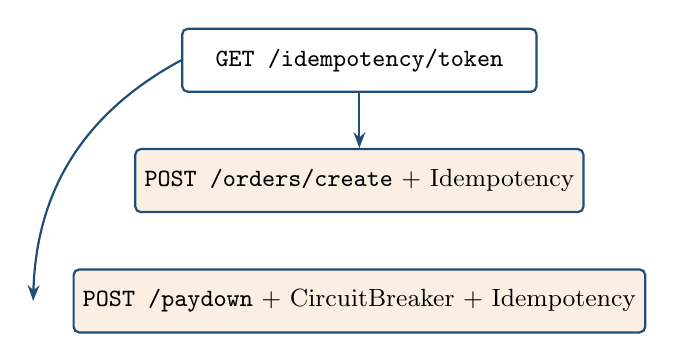
\begin{tikzpicture}[node distance=7mm]
  \node[node-box,minimum width=45mm] (token) {\small \texttt{GET /idempotency/token}};
  \node[node-box,below=of token,minimum width=45mm,fill=cAccent!12] (order) {\small \texttt{POST /orders/create} + Idempotency};
  \node[node-box,below=of order,minimum width=45mm,fill=cAccent!12] (pay) {\small \texttt{POST /paydown} + CircuitBreaker + Idempotency};

  \draw[arrow] (token) -- (order);
  \draw[arrow,bend right=30] (token.west) to ([xshift=-5mm]pay.west);
\end{tikzpicture}
\vspace{2mm}
\small 两个"花钱接口"都强制带 Idempotency-Key —— 没有 key 直接拒绝。
\srcnote{routes/router.go:74 颁发 / routes/router.go:77 下单 / routes/router.go:102 支付}
\end{frame}

\begin{frame}{TTL 为什么定 5 分钟}
\begin{itemize}
  \item 业务窗口：从打开下单页到点支付，正常用户 30 秒到 2 分钟。
  \item 重试窗口：Nginx 默认 \texttt{proxy\_connect\_timeout=60s}，移动端 SDK retry 3 次约 6--15 秒。
  \item 用户切应用/锁屏 $\to$ 回来再点，常见 2--3 分钟。
  \item 5 分钟覆盖以上所有正常场景，又不至于让 Redis 长期累积 key。
\end{itemize}
\vspace{2mm}
\small 太短 $\to$ 提早过期，重试变新请求 $\to$ 真的重复扣款。
\small 太长 $\to$ 内存涨 + token 泄漏窗口拉大。
\srcnote{repository/cache/idempotency.go:16 \texttt{IdempotencyTokenTTL = 5 * time.Minute}}
\end{frame}

% ============== 5. 业务侧 trade-off ==============
\section{业务侧 trade-off}

\begin{frame}{失败回滚到 init：把"重试权"还给用户}
\begin{itemize}
  \item 业务返回 4xx/5xx 时，中间件把状态从 \texttt{processing} 打回 \texttt{init}。
  \item 业务含义：服务端承认"我没把你这次意图做成功"，允许用户用同一 token 重试。
  \item 反例：如果失败也写 \texttt{done}，那用户的"提交"就被吞了 —— 钱没扣，订单也没生成，但 token 锁死。
  \item 用户的反应：找客服。客服找研发。研发翻日志。一次重复扣款的成本就此发生在一次"看似没扣款"的请求上。
\end{itemize}
\srcnote{middleware/idempotency.go:101--105 释放路径}
\end{frame}

\begin{frame}{为什么不"锁死 token 直到客户端确认"}
\begin{tabular}{@{}lll@{}}
\toprule
策略 & 用户体验 & 平台成本 \\
\midrule
失败回滚到 init & 重试无感，自然 & 偶尔多算一次 \\
锁死 token 等 ack & 用户被卡住要刷新 & 客服话务高 \\
直接删除 token & 重试变新请求 & 真重复扣款 \\
\bottomrule
\end{tabular}
\vspace{2mm}
\keypoint{"宽容失败 + 严格成功"——失败可重试，成功必回放。}
\end{frame}

\begin{frame}{客户端不重试，token 怎么办？}
\begin{itemize}
  \item 真实场景：用户点完提交就关掉 App，不再回来。
  \item token 留在 Redis 里，TTL 5 分钟自然过期，无人工干预成本。
  \item 不需要客户端"主动注销"——简化了 API 也免除了"销毁失败"再次重复扣款的边界 case。
\end{itemize}
\vspace{2mm}
\keypoint{TTL 是 token 生命周期的"兜底回收器"，不是缓存的副产品。}
\srcnote{repository/cache/idempotency.go:53--60 颁发即设 TTL}
\end{frame}

\begin{frame}{Redis 挂了：业务侧怎么决策？}
\begin{itemize}
  \item 选项 A：放行业务（fail-open）—— 体验好，但失去幂等保护，真重复扣款。
  \item 选项 B：拒绝请求（fail-close）—— 钱相关接口默认安全；用户看到"系统繁忙"远好过"被扣两次"。
  \item gomall 选 B：Lua 出错直接返回 5xx，不进业务。
\end{itemize}
\vspace{2mm}
\small 这不是技术选型，是"用户钱袋"和"系统可用性"的取舍 —— 钱永远优先。
\srcnote{middleware/idempotency.go:61--69 fail-close 实现}
\end{frame}

% ============== 6. 压测验证 ==============
\section{压测验证：755K 请求只扣一笔}

\begin{frame}{业务承诺的量化证据}
\small
\begin{tabular}{@{}lr@{}}
\toprule
指标 & 数值 \\
\midrule
压测脚本 / VU / 时长 & \texttt{idempotency\_replay.js} / 50 / 15s \\
\textbf{累计请求} & \textbf{755{,}033} \\
\textbf{DB 实际订单} & \textbf{1} \\
\textbf{回放路径 p95 / RPS} & \textbf{2.33ms} / 50{,}319 \\
错误率 & 0\% \\
\bottomrule
\end{tabular}
\vspace{2mm}
\keypoint{75 万次"用户狂点提交"，账上只多了一笔订单 —— 这就是幂等保护的业务量化。}
\srcnote{stressTest/REPORT.md \S 4. 幂等中间件：755K 请求 → 1 笔订单}
\end{frame}

\begin{frame}{业务侧的换算：一笔订单防住多少客诉}
\begin{itemize}
  \item 假设 50 个并发 VU 模拟"双 11 凌晨同一用户狂点 + Nginx 重试"，15 秒打出 75 万次。
  \item 没有幂等 $\to$ 理论上 75 万笔订单 + 75 万次扣款，全部需要客服退款。
  \item 有幂等 $\to$ 1 笔订单，0 笔重复扣款，0 个工单。
  \item 客服人工 + 退款手续费节省：单一用户单一时段就是\textbf{万元级}。
\end{itemize}
\srcnote{stressTest/REPORT.md \S 链路压测表 第 4 行}
\end{frame}

% ============== 7. 业界对比 ==============
\section{业界对照：Stripe / 支付宝 / 微信支付}

\begin{frame}{Stripe：把 Idempotency-Key 写进 API 规范}
\begin{itemize}
  \item Stripe 在 2015 年公开博客《Designing robust and predictable APIs with idempotency》里定义了 \texttt{Idempotency-Key} 头部。
  \item 规范：客户端生成 UUID，传给所有"非幂等"操作（POST charges、POST refunds）。
  \item 服务端保留请求结果 24 小时，期间同 key 重发直接回放。
  \item 后来成为 IETF 草案 \texttt{draft-ietf-httpapi-idempotency-key-header}（行业事实标准）。
\end{itemize}
\vspace{2mm}
\small gomall 的设计是这条规范的最小实现：header 名相同 (\texttt{Idempotency-Key})，语义相同（回放上次结果）。
\end{frame}

\begin{frame}{支付宝 / 微信支付：同类设计，名字不同}
\begin{tabular}{@{}lll@{}}
\toprule
平台 & 字段名 & 业务语义 \\
\midrule
Stripe & \texttt{Idempotency-Key} (Header) & 客户端生成，24h TTL \\
支付宝 & \texttt{out\_trade\_no} (商户订单号) & 商户保证唯一，不重复 \\
微信支付 & \texttt{out\_trade\_no} (商户订单号) & 同上 \\
gomall & \texttt{Idempotency-Key} (Header) & 服务端颁发，5min TTL \\
\bottomrule
\end{tabular}
\vspace{2mm}
\small 三家做法本质一样：服务端把"业务意图"绑死到一个不可变 key 上，重复提交一律回放。
\srcnote{微信支付/支付宝商户文档均要求 \texttt{out\_trade\_no} 在商户系统内唯一}
\end{frame}

\begin{frame}{设计差异：客户端生成 vs 服务端颁发}
\begin{tabular}{@{}lll@{}}
\toprule
方案 & 优点 & 缺点 \\
\midrule
客户端生成 (Stripe) & 离线可用、无往返 & 必须信任客户端不重用 \\
服务端颁发 (gomall) & 强约束、按用户隔离 & 多一次 RTT \\
商户号即 key (支付宝) & 业务自然 key，可对账 & 商户需自己保证不重复 \\
\bottomrule
\end{tabular}
\vspace{2mm}
\small gomall 选服务端颁发的原因：C 端用户的客户端实现不可控，UUID 重用风险高 —— 多一次 RTT 换严格性，值。
\end{frame}

% ============== 8. Q&A ==============
\appendix

\begin{frame}{Q\&A：业务侧 + 技术侧}
\scriptsize
\textbf{业务 Q1}：用户钱被扣两次，平台一次综合成本大概多少？\\
\hspace{3mm}A：单笔约 10 元（手续费 + 客服 + 资金占用），日均 500 起 $\approx$ 年 180 万。

\vspace{0.8mm}
\textbf{业务 Q2}：为什么 token 用服务端颁发，不让前端生成 UUID？\\
\hspace{3mm}A：前端实现不可控，重用风险高；服务端颁发可按用户隔离、可强约束 TTL。

\vspace{0.8mm}
\textbf{业务 Q3}：TTL 为什么是 5 分钟，不是 1 小时？\\
\hspace{3mm}A：覆盖正常下单到支付窗口 + 网络重试；更长会增加泄漏风险与 Redis 内存。

\vspace{1.5mm}
\textbf{技术 Q1}：Nginx \texttt{proxy\_next\_upstream} 会重发 POST 吗？\\
\hspace{3mm}A：默认 \texttt{error timeout} 包含 POST；服务端必须假设"POST 也可能重复"。

\vspace{0.8mm}
\textbf{技术 Q2}：失败回滚到 init 和"删 token"有什么区别？\\
\hspace{3mm}A：回滚到 init 允许同 key 重试；删 token 让重试变新请求，直接破坏幂等。

\vspace{0.8mm}
\textbf{技术 Q3}：跟支付宝 \texttt{out\_trade\_no} 比，gomall 设计本质区别？\\
\hspace{3mm}A：本质相同（意图绑死 key）；差异在颁发方与生命周期（客户端长期 vs 服务端 5min）。
\end{frame}

\begin{frame}{代码位置与参考来源}
\textbf{gomall 实现}
\begin{description}\small
  \item[中间件主干]\srcnote{middleware/idempotency.go:35--112}
  \item[Lua 状态机]\srcnote{repository/cache/idempotency.go:32--50}
  \item[失败回滚]\srcnote{middleware/idempotency.go:101--105 + repository/cache/idempotency.go:87--90}
  \item[token 颁发]\srcnote{api/v1/idempotency.go:16--46}
  \item[按用户隔离 key]\srcnote{repository/cache/key.go:15--21}
  \item[路由挂载]\srcnote{routes/router.go:74 / :77 / :102}
  \item[压测脚本与数据]\srcnote{stressTest/idempotency\_replay.js / stressTest/REPORT.md \S 4}
\end{description}

\vspace{2mm}
\textbf{业界参考}
\begin{description}\small
  \item[Stripe API] \texttt{Idempotency-Key} 设计博客（2015，官方）
  \item[IETF 草案] \texttt{draft-ietf-httpapi-idempotency-key-header}
  \item[支付宝/微信支付] 商户 API 文档中的 \texttt{out\_trade\_no} 唯一性要求
\end{description}
\end{frame}

\end{document}
